\documentclass[./Thesis]{subfiles}


\graphicspath{{./Images/}}

\begin{document}

\chapter{Introduction to the Muon G-2 Experiment}

The muon g-2 experiment has a long history of the associated science associated with it. In the following sections I will explain the history of the experiment and where this experiment comes from along with the fundamental idea of this experiment.  Furthermore, I will explain the results that were done in the previous experiment E821 and how this relates to standard model predictions which give the fundamental reasoning for performing E989 the current G-2 experiment. Everything in this chapter is paraphrased from Ref. \cite{TDR} which give the best introductory information on the experiment.

\section{History and Motivation}


The muon anomalous magnetic moment has been measured in a series of experiments at Cern and more recently in the E821 experiment at the BrookHaven National Laboratory. In the first Cern measurements muons were injected into a 6-m long straight magnet where they followed a drifting spiral path, slowly traversing the magnet because of a small gradient introduced in the field. The muons were topped in a polarimeter outside the magnet and the measurement of their net spin precession determined $a_\mu$ with an uncertainty of 4300 ppm. The results agreed with the prediction of QED for a structureless particle. The second Cern experiment used a magnetic ring to extend the muon storage time. The muon precession frequency was measured by the number of decayed positrons vs. time and observing the precession frequency of the decayed positrons. They were able to determine the value of $a_\mu$ to an uncertainty of 270 ppm, which agreed with theory only after the value had to be recalculated. Furthermore, the third Cern experiment also used a magnetic storage ring with a much higher rate and was able to determine $a_\mu$  within an uncertainty of 10 ppm, which also agreed with theory. The most recent Brook Haven Experiment followed the same principles as the third Cern experiment but having multiple improvements in the field uniformity and increased storage efficiency, they were able to determine $a_\mu$  to an uncertainty of 0.54 ppm. Ref. \cite{TDR}

\subsection{Magnetic and Electric Dipole Moments}

	The study of magnetic moments started with the development of quantum mechanics. For fermions it is related to the spin by 
	
	\begin{equation}\label{EQ:MDM}
	\vec{\mu} = g \frac{Qe}{2m} \vec{s}
	\end{equation}
	
In our modern interpretation of the Stern-Gerlach experiment is that their observations was telling us that the g-factor of the unpaired electron in 2.  However, coming to this conclusion required the discovery of the spin, quantum mechanics, along w/ Thomas' relativistic correction. Following this Dirac's relativistic theory predicts that $g=2$. In 1933 Stern showed that that the g-factor of the proton was approximately 5.5 which proved that the proton was not a pure Dirac particle. In addition, Alvarez and Bloch discovered the the neutron had a large magnetic moment which was not expected.

In 1947, motivated by measurements of the hyperfine structure in hydrogen, which obtained the splitting are larger than expected from Dirac theory, Schwinger showed that from a theoretical standpoint this splitting can be accounted for by adding in a term for the electron spin magnetic moment for the lowest radiative correction to the Dirac moment.

	\begin{equation}
	\frac{\delta\mu}{\mu}  = \frac{1}{2 \pi } \frac{e^2}{\hbar c}
	\end{equation}
	
It has been found useful to break the magnetic dipole moment into two terms as follows.\cite{TDR}
	
	\begin{equation}
	\mu = (1+a)\frac{e\hbar}{2m}
	\end{equation}
	Where
	\begin{equation}
	a = \frac{g-2}{2}
	\end{equation}
	
	
\subsection{The Muon}

	The muon was first observed in a Wilson cloud chamber by Kunze in 1933. In 1936, Anderson and Neddermeyer reported that the muon is less massive than the proton but more penetrating than the electron. The Yukawa theory of the nuclear force predicted such a particle which interacted to weakly with matter to be the carrier of the nuclear force. Muon decays through the nuclear force $e^+ \rightarrow e^{-}\nu_{\mu}\overline{\nu}_{e}$ in which the muons long lifetime of approximately 2.2 ns permits precession measurements of its mass, lifetime, and magnetic moment which makes it a good candidate for experiments.Ref. \cite{TDR}

\subsection{The Muon Magnetic Moment}

	The muon magnetic moment played an important role in the discover of the generation structure of the standard model. The muon spin experiment at Nevis Cyclotron observed parity violation in muon decays, in addition to showing that $g_\mu$ is consistent with 2. Subsequent experiments showed that $a_\mu \equiv \frac{\alpha}{2\pi} $ implying that in a magnetic field the muon behaves like a heavy electron.Ref. \cite{TDR}


\subsection{The Muon Electric Dipole Moment}


	Dirac discovered an EDM term in his relativistic theory and like the magnetic dipole moment, the EDM must be in the direction of the spin. The equation for the Electric dipole moment is given by Eq. \ref{EQ:EDM}
	
	\begin{equation}\label{EQ:EDM}
		\vec{d} = \eta (\frac{Qe}{2mc}) \vec{s}
	\end{equation}

	Where $\eta$ is dimensionless and analogous to g in Eq. \ref{EQ:MDM}. An EDM is forbidden by parity and by time reversal which was first pointed out by Landau and Ramsey by examining the hamiltonian \ref{EQ:Hamiltonian}
	
	\begin{equation}\label{EQ:Hamiltonian}
	H = -\vec{\mu} \cdot \vec{B} - \vec{d} \cdot \vec{E}
	\end{equation}
	
Therefore searches for a permanent EDM of electrons, neutrons, and atomic nucleus have become an important search for physics beyond the standard model.Ref. \cite{TDR}

\section{Quick Summary of Experimental Technique}

	In E989 a polarized beam of muons are produced and injected into a storage ring from the main Fermilab ring. The magnetic field is a dipole field in the storage ring with vertical focussing being provided by the electrostatic quadrupoles. There are two frequencies are measured experimentally, the first frequency $\omega_{a}$ is the rate at which the muon polarization turns relative to the momentum of the muon, and the second frequency $\omega_p$ is the value of the magnetic field normalized to the Larmour frequency.
	
	\begin{equation}
	\vec{\omega}_{a} = \vec{\omega}_{S} - \vec{\omega}_{C}
	\end{equation}

Where S denotes the spin and C denotes the cyclotron which the individual terms are given by Eq.'s \ref{EQ:omegaS} and \ref{EQ:omegaC}

	\begin{equation}\label{EQ:omegaS}
	\omega_{S} = -g \frac{Qe}{2m} B - (1-\gamma)\frac{Qe}{\gamma m} B
	\end{equation}

	\begin{equation}\label{EQ:omegaC}
	\omega_C = - \frac{Qe}{m\gamma} B
	\end{equation}

It is worth noting that $\omega_a$ depends only on the anomoly $a_\mu$ and depends linearly on the applied magnetic feild.

In the presence of an electric field we get \ref{EQ:omegaA}

\begin{equation}\label{EQ:omegaA}
\vec{\omega}_a = -\frac{Qe}{m}[a_{\mu} \vec{B} + (a_{\mu} - (\frac{m}{p})^2) \frac{\vec{\beta} \times \vec{E}}{c}]
\end{equation}


If $p_{magic} = \frac{m}{\sqrt{a_\mu}} \equiv 3.09 \frac{Gev}{c}$ the electric feild contribution in Eq. \ref{EQ:omegaA} cancels to the 1st order which only requires higher order corrections to the term. The factor $a_\mu$ from the 2 frequencies we use the relation \ref{EQ:amu}

\begin{equation}\label{EQ:amu}
a_\mu = \frac{\omega_a / \omega_p}{\lambda_{+} - \omega_a / \omega_p}
\end{equation}

The necessary steps in the experiment consist of the following.Ref. \ref{TDR}


1.	Production of an appropriate pulsed proton beam from accelerator complex.

2.	Production of pions using the proton beam that has been prepared.

3. 	Collection of the polarized muons from pion decay.

4.	Transporting GM2 storage ring.

5. 	Injection of the muon beam into the storage ring.

6. 	Kicking the muon beam onto stored orbits

7.	Measuring the arrival time and energy of positrons form the muon decays.


\vspace{5mm}

\subsection{Quick Introduction to Muon Beam Dynamics}

Here is given a quick introduction to the physics of the beam dynamics of a weakly focused betatron which is used in the current E989 experiment. This section is mainly used to give an introduction to the pitch correction and the radial field correction which will be talked about later in the systematics study. 

Beam dynamics of the storage ring directly affects the measurement of $a_\mu$ since the detector acceptance for the decay electrons depends on the radial coordinate of the muon at the point where it decays. Resonances in the storage ring also can cause particle losses which affect the measurement. Care is taken in the experiment in setting the frequency of the coherent betatron oscillation which lies close to the second harmonic $f_a = \omega_a / 2\pi$. If $f_{cbo}$ is to close to $2*f_a$ , which is the beat frequency, this complicates the extraction of $f_a$ from the data and can introduce significant systematical error.
	A pure quadrupole electric field provides a linear restoring force in the vertical direction and the combination of the electric filed and the central magnetic field provides a linear restoring force in the radial direction. The g-2 storage ring is a weak focusing ring with the field index
	
	\begin{equation}
	n =\frac{\kappa R_0}{\beta B_0}
	\end{equation}

	Where $\kappa$ is the electric quadrupole gradient, $B_0$ is the magnetic field strength, $R_0$ is the magic radius, and $\beta$ is the relativistic velocity of the muon beam.  For a ring with a uniform vertical dipole magnetic field and a uniform quadrupole field the horizontal and vertical motion is given by \ref{EQ:VerticalCBO} \ref{EQ:horizontalCBO}.
	
	\begin{equation}
	\label{EQ:VerticalCBO}
	x = x_e +A_x cos(\nu_x \frac{s}{R_0} + \delta_x)
	\end{equation}


	\begin{equation}
	\label{EQ:horizontalCBO}
	y =  A_y cos(\nu_y \frac{s}{R_0} + \delta_y)
	\end{equation}
Where s is the arc length along the trajectory of the ring. The horizontal and vertical tunes are given by \ref{EQ:verticalTune} \ref{EQ:horizontalTune}.

	\begin{equation}
	\label{EQ:verticalTune}
	\nu_x = \sqrt{1-n}
	\end{equation}

	\begin{equation}
	\label{EQ:horizontalTune}
	\nu_y = \sqrt{n}
	\end{equation}
In E821 there were several tunes used for in the data acquisition $n = 0.137, 0.142, 0.122$. The horizontal and vertical betatron frequencies are given by \ref{EQ:verticalFreq} \ref{EQ:horizontalFreq}.

	\begin{equation}
	\label{EQ:verticalFreq}
	f_x = f_c \sqrt{1-n} \equiv 0.929 f_c
	\end{equation}
	
	\begin{equation}
	\label{EQ:horizontalFreq}
	f_y = f_c \sqrt{n} \equiv 0.37f_c
	\end{equation}

Where $f_c$ is the cyclotron frequency and $n=0.137$. The field index also determines the angular acceptance of the ring where the maximum horizontal and vertical angle of the muon momentum are given by \ref{EQ:verticalAngle} \ref{EQ:horizontalAngle}

	\begin{equation}
	\label{EQ:verticalAngle}
	\theta^{x}_{max} = \frac{x_{max} \sqrt{1-n}}{R_0}
	\end{equation}

	\begin{equation}
	\label{EQ:horizontalAngle}
	\theta^{y}_{max} = \frac{y_{max} \sqrt{n}}{R_0}
	\end{equation}

Where $x_{max} ,y_{max} =  45mm$ which is the radius of the storage ring aperture.

For a ring with discrete quads the focusing strength changes as a function of azimuth and the equation of motion looks like an oscillator where the spring constant constantly changes as a function of azimuth s. 

	\begin{equation}
	X(s) = x_e + A \sqrt{\beta(s)} cos(\phi(s)+\delta)
	\end{equation}
The presence of the coherent betatron oscillation was first discovered in the E821 experiment from a plot that showed there was in azimuthal variation in $a_\mu$ so this leaded to a correction factor.

n the simplest case, in the absence of an electric field and when the velocity is perpendicular to the magnetic field the rate at which the spins turns relative to the momentum is given by \ref{EQ:omegaA}.
	
	\begin{equation}
	\label{EQ:omegaA}
	\omega_{a} = -a\frac{Qe}{m} B
	\end{equation}

However, in the real experiment not all the muons are at the magic momentum, therefore a precision knowledge of the trajectories required. To look at this effect we calculate the effect on the electric field due to muon not directly $\gamma_{magic}$, for the moment neglecting the $\vec{\beta}\cdot\vec{B}$ terms.

	\begin{equation}
	\omega_{a}' = \omega_{a}[1-\beta\frac{E_r}{B_y}(1-\frac{1}{a_\mu \beta^2 \gamma^2})]
	\end{equation}

Where $\omega_{a} = -a \frac{Qe}{m}B$. Now using the fact that $p=\beta\gamma m = p_m + \Delta p$ we get \ref{EQ:deltaomega}.


\begin{equation}
\label{EQ:deltaomega}
\frac{\Delta \omega_a}{\omega_a} = -2 \frac{\beta E_r}{B_y}(\frac{\Delta P}{P_m})
\end{equation}

Where the fractional change in momentum in \ref{EQ:deltaomega} can be represented as \ref{EQ:deltap}

\begin{equation}
\label{EQ:deltap}
\frac{\Delta P}{P_m}=(1-n)\frac{\Delta R}{R_0} = (1-n) \frac{X_e}{R_0}
\end{equation}

Where the $X_e$ is the muons beam equilibrium radius. Then the Electric quadrapole field is given by \ref{EQ:Efield}

\begin{equation}
\label{EQ:Efield}
E = \kappa X = \frac{n\beta B_y}{R_{0}}x
\end{equation}

Therefore we obtain the final result to the change in frequency \ref{EQ:deltaw}.

\begin{equation}
\label{EQ:deltaw}
\frac{\Delta \omega}{\omega} = -2n(1-n)\beta^2\frac{x x_e}{R_0^2 B_y}
\end{equation}

Therefore, the effect of muons not at the magic momentum is to lower the measured $\omega_a$ frequency. For a quadrapole focusing feild plus a uniform magnetic field the time average of $<x> = x_e$, so the electric field correction is given by \ref{EQ:EFieldCorrection}. The value $<x_e^2>$ is determined in the fast rotation analysis which will not be covered in this thesis. In the Brookhaven experiment it was found for a low n that $C_E = 0.47 \pm 0.054 ppm$.

\begin{equation}
\label{EQ:EFieldCorrection}
C_E = \frac{\Delta\omega}{\omega} = -2n(1-n)\beta^2\frac{<x_e^2>}{R_0^2 B_y}
\end{equation}


The betatron oscillations of the muon beam lead to the terms $\vec{\beta}\cdot\vec{B}\neq0$. Since the $\vec{\beta}\cdot\vec{B}$ term is quadratic in the component of $\vec{\beta}$, its contribution to $\vec{\omega_s}$ will not generally average out to zero. The spin precession frequency has a small dependence on the betatron motion of the beam, and it turns out the only significant correction comes from the vertical betatron oscillations which is called the pitch correction. The pitch angle varies harmonically as in \ref{EQ:betatron}

\begin{equation}
\label{EQ:betatron}
\psi = \psi_0 Cos(\omega_y t)
\end{equation}


Where $\omega_y$ is the vertical betatron frequency. If we set $a_\mu - \frac{1}{\gamma^2-1}=0$ we obtain \ref{EQ:omegaDiff}

\begin{equation}
\label{EQ:omegaDiff}
\vec{\omega}_{diff} = - \frac{Qe}{m}[a_\mu \vec{B} - a_\mu(\frac{\gamma}{\gamma+1})(\vec{\beta}\cdot\vec{B})\vec{\beta}]
\end{equation}

Now if we assume that the pitch angles are small, and $\vec{B} = \hat{y} B_y$ and $\beta=\hat{z}\beta_z + \hat{y}\beta_y$ we get the difference in frequency \ref{EQ:oDiff}

\begin{equation}
\label{EQ:oDiff}
\omega_{ay}' = -\omega_a[1-(\frac{\gamma -1 }{\gamma})\psi^2]
\end{equation}


This then gives the pitch correction \ref{EQ:pitchCorrection}

\begin{equation}
\label{EQ:pitchCorrection}
C_p = - \frac{<\psi^2>}{2} = - \frac{n}{4}\frac{<y^2>}{R_0^2}
\end{equation}

The result that the pitch correction and the radial field corrections are dependent on the average positions is what makes straw trackers important in GM2 since these detectors have the best resolution for position measurements. 

\section{Results from E821 Experiment}
	The Brookhaven based experiment E821 which was completed in 2001 was a very successful experiment in its achievements. As previously said they were able to measure the precession frequency to approximately 14 times better than what was ever achieved before in the previous cern experiments. Steady improvements in the theory resulted in a present measurement of $a_\mu$ with an uncertainty of 0.42 ppm. The E821 experiment was able to reach a field uniformity to $\pm1$ ppm uniformity on average. The main systematical uncertainties of this experiment were from anything the caused the extracted frequency to vary the the true fit value. Uncertainties in $\omega_a$ measurement mainly consist of gain instability in the detectors, lost muons, spin tracking, coherent betatron oscillations, differential decays, pitch correction uncertainties. The main source of uncertainty from the $\omega_p$ measurement consist of errors due to non uniformity in the magnetic field. The results for E821 are given in Fig. \ref{fig:E821Results} which show previous measurements and the Standard Model Predictions which shows that there was a discrepancy from standard model values for $a_\mu$ and the BrookHaven measured values up to 3.5 sigma. Ref.\cite{TDR}
	
\begin{figure}
\centerline{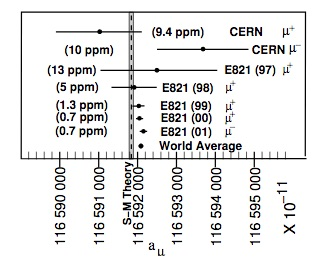
\includegraphics[height=95mm]{E821Result.jpg}}
\caption[$a_\mu$ results after E821]{ Measurement of $a_\mu$ from CERN and BNL E821. The vertical band in the SM value using the hadronic contribution. \cite{TDR}
	}
\label{fig:E821Results}
\end{figure}



\end{document}